\chapter{DishBrain}
\chaptermark{DishBrain}
\label{sec:dishbrain}
\begin{chaptergoals}
\item how DishBrain codes the ball by place and rate and reads the paddle as a count difference;
\item why a count in a $10\ms$ window is noisy, so the network can shift only the mean;
\item how shaking the network only after misses drifts it toward configurations that fail less;
\item what was measured, what is disputed, and how to rebuild the bench to test the mechanism.
\end{chaptergoals}

\section{A network in a dish plays tennis}

DishBrain is the name its authors gave to a bench on which a culture of living neurons, grown on a chip with electrodes, plays a simplified one-paddle tennis game~\cite{Kagan2022}. It is the most discussed experiment with a machine made of living neurons (such machines are surveyed in Chapter~\ref{sec:livingmachine}), and it is especially convenient for this book. Here a small network is accessible in its entirety: the experimenter sets every input, and every output is recorded. All the questions of the preceding chapters, how the signal is encoded, who teaches, what the probe sees, can be put to a network that has no eyes, no muscles, and no \nt{DOPA} neurons. Let us take the experiment apart the way an engineer takes apart someone else's bench: circuit, input, output, teacher, result, disputes.

\section{The bench}

The neurons are taken from embryonic mouse cortex, about $800\,000$ cells per chip, or grown from human stem cells, about a million per chip. For several weeks they grow on the chip, grow into one another, and begin to produce spikes and bursts on their own. Beneath them, on an $8$~mm$^2$ area, lie $26\,000$ platinum electrodes; up to $1024$ of them can be recorded at once, and in practice stimulation goes through eight.

A loop is closed around the culture (Fig.~\ref{fig:dishloop}). A computer simulates the game: the ball flies, bounces off the walls, and the paddle moves up and down. The ball position is turned into current on eight ``sensory'' electrodes. Spikes from two ``motor'' regions are counted in $10\ms$ windows and move the paddle. After each hit or miss the culture receives one more stimulus, the feedback. The $10\ms$ windows are the clock of the bench computer, not of the culture: the network itself still runs asynchronously, like every network in this book.

\begin{figure}[t]
\centering
\begin{tikzpicture}[>=Stealth,
  blk/.style={draw,very thick,rounded corners=3pt,align=center,font=\small,minimum height=1.2cm},
  lab/.style={font=\scriptsize,align=center}]
\node[blk,fill=blue!6,text width=3.4cm] (C) at (0,0) {culture on a chip\\\scriptsize $\sim10^6$ neurons, $26\,000$ electrodes};
\node[blk,fill=orange!10,text width=3.0cm] (G) at (7.2,0) {computer:\\tennis game};
\draw[->,very thick,blue!60!black] (G.north west) to[bend right=25] node[lab,above] {ball: \emph{place} = which of 8 electrodes,\\\emph{rate} = 4--40 spikes/s} (C.north east);
\draw[->,very thick,red!70!black] (C.south east) to[bend right=25] node[lab,below] {paddle: spike counts of the\\``up'' and ``down'' regions per $10\ms$} (G.south west);
\draw[->,thick,densely dashed,green!45!black] (G.east) -- ++(0.9,0) |- ++(0,-2.6) -| node[lab,pos=0.25,below] {hit: predictable stimulus; miss: unpredictable} (C.south);
\end{tikzpicture}
\caption{The DishBrain loop. Blue arrow: input; the ball position is encoded by a place code and a rate code (Chapter~\ref{sec:code}). Red: output; the difference between the counts of two regions moves the paddle. Green dashed: feedback after each rally, the bench's only ``teacher.''}
\label{fig:dishloop}
\end{figure}

\section{Input and output}

The \emph{input} is written in two codes of Chapter~\ref{sec:code} at once. Which of the eight electrodes is stimulated tells how high the ball is: this is a place code, like that of the sensors in Chapter~\ref{sec:sensors}. How often the stimulation pulses come tells how far away the ball is: $4$ per second when it is at the far wall, rising linearly to $40$ per second when it is at the paddle's wall. This is a rate code; the amplitude of the ball pulses is $75$~mV. The culture does not ``know'' either code in advance: the code is set by the experimenter, and the network has to learn to read it.

The \emph{output} is read the same way as in the interfaces of Chapter~\ref{sec:debugging}. Spikes of one motor region push the paddle up, those of the other push it down; in the simplest form, for each window,
\begin{empheq}[box=\keybox]{equation}
\Delta p \;=\; c\,\bigl(n_\uparrow - n_\downarrow\bigr),
\label{eq:dishreadout}
\end{empheq}
where $n_\uparrow$, $n_\downarrow$ are the spike counts of the two regions in $10\ms$, and $c$ is a bench constant. This is the two-wire code of Chapter~\ref{sec:glutcomputer}: the direction of movement is carried not by the sign of a signal but by which of the two wires is louder.

Consider the noise of such an output. If a region emits a total of $R$ spikes per second, a window $T=10\ms$ holds $RT$ of them on average, and by~\eqref{eq:rateerror} the relative spread is $1/\sqrt{RT}$. At $R=1000$ spikes per second this is about $30$ percent in each window; at $R=100$, more than a hundred. The paddle inevitably jitters, and the network can learn in only one way: by shifting the \emph{mean} count difference in the right direction. These are the same laws that limit any interface of Chapter~\ref{sec:debugging}, only now on both sides of the loop.

\section{A teacher without dopamine}

The most interesting part of the bench is the teacher. A culture of cortical neurons has no \nt{DOPA} neurons, and the bench sends no ``better than expected'' signal. The feedback is different. If the network hits the ball, a short \emph{predictable} stimulus goes to all eight sensory electrodes at once: $75$~mV pulses at $100$ per second for $0.1\,\text{s}$. If it misses, for four seconds it receives a stimulus the authors call \emph{unpredictable}: $150$~mV pulses at $5$ per second, at random times, on randomly chosen electrodes; then four seconds of pause without stimulation, and the ball starts again~\cite{Kagan2022}.

The authors started from the hypothesis that the network acts so as to make its input predictable~\cite{Friston2010}. For an engineer the meaning is simple: the culture has exactly one way to get rid of four seconds of random noise, which is to hit the ball. We met the same idea in the spike economy of Chapter~\ref{sec:code} and in frame prediction in Chapter~\ref{sec:recognition}.

But is predictability really what is needed here? A cruder mechanism is possible. Suppose the unpredictable stimulus after a miss simply \emph{scrambles} recent changes in the network, while the calm stimulus after a hit leaves them alone. Describe the network's configuration by a single vector $\boldsymbol\psi$, and let the network miss with probability $P_{\text{miss}}(\boldsymbol\psi)$ in configuration $\boldsymbol\psi$. If the kicks are symmetric, so that going from $\boldsymbol\psi$ to $\boldsymbol\psi'$ is as likely as the reverse, then in steady state the outflow from each configuration balances the inflow, and the fraction of time the network spends in configuration $\boldsymbol\psi$ is
\begin{empheq}[box=\keybox]{equation}
\rho(\boldsymbol\psi) \;\propto\; \frac{1}{P_{\text{miss}}(\boldsymbol\psi)} .
\label{eq:dishdensity}
\end{empheq}
A configuration that misses ten times less often is held ten times longer. No one tells the network which way to change its weights: good configurations are simply destroyed less often.

We tested this on a model that reduces the culture to two numbers: the paddle arrives at the point $a\,y+b$ when the ball arrives at height $y$, and it hits if it misses by less than $0.1$. After a miss both numbers get a random kick; after a hit they stay the same. The fraction of hits over $2000$ rallies grew from $0.21$ in the first two hundred to $0.38$ in the last five hundred (forty ``cultures,'' Fig.~\ref{fig:dishmodel}). If the kick is given after \emph{every} rally, the feedback carries no information, and the fraction stays around $0.12$; if there are no kicks at all, it stays at $0.19$. The bench experiment agrees with this: a significant improvement within a session appeared only with full feedback. With silence in place of the stimuli the culture still played better by the end of the session than without feedback, but with a smaller effect~\cite{Kagan2022}; note that in this condition, too, a miss is followed by a long pause and a hit by a short one, so the difference between outcomes does not vanish entirely.

\begin{figure}[t]
\centering
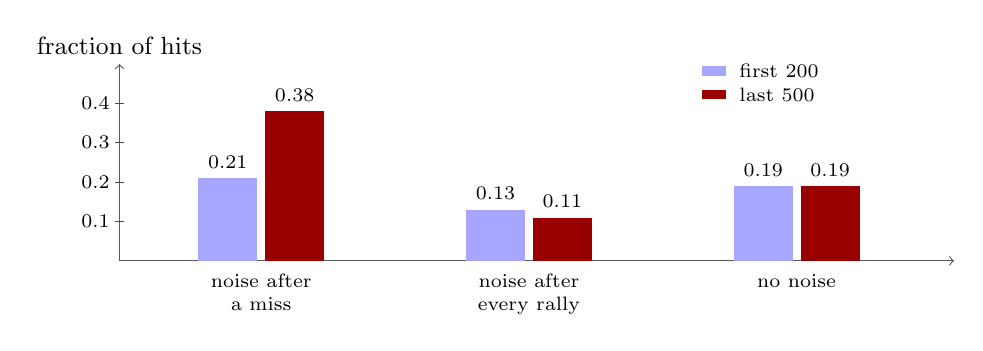
\begin{tikzpicture}[x=1cm,y=5cm]
\draw[->,gray!70!black] (0,0) -- (10.6,0);
\draw[->,gray!70!black] (0,0) -- (0,0.5) node[above,font=\small,black] {fraction of hits};
\foreach \v in {0.1,0.2,0.3,0.4}{\draw[gray!60!black] (-0.06,\v) -- (0.06,\v); \node[left,font=\scriptsize] at (0,\v) {\v};}
\foreach \x/\f/\l/\lab in {1.8/0.21/0.38/{noise after\\a miss},5.2/0.13/0.11/{noise after\\every rally},8.6/0.19/0.19/{no noise}}{
  \fill[blue!35] (\x-0.8,0) rectangle (\x-0.05,\f);
  \fill[red!60!black] (\x+0.05,0) rectangle (\x+0.8,\l);
  \node[below,font=\scriptsize,align=center] at (\x,-0.01) {\lab};
  \node[above,font=\scriptsize] at (\x-0.425,\f) {\f};
  \node[above,font=\scriptsize] at (\x+0.425,\l) {\l};}
\fill[blue!35] (7.4,0.47) rectangle (7.7,0.495); \node[right,font=\scriptsize] at (7.75,0.482) {first 200};
\fill[red!60!black] (7.4,0.41) rectangle (7.7,0.435); \node[right,font=\scriptsize] at (7.75,0.422) {last 500};
\end{tikzpicture}
\caption{The ``scramble on a miss'' model (\texttt{dishbrain\_model.py}): fraction of hits at the start and at the end of $2000$ rallies, averaged over forty model cultures. Learning occurs only if the kick follows a miss and not a hit, as in the experiment, where a significant improvement within a session appeared only with full feedback.}
\label{fig:dishmodel}
\end{figure}

\begin{keyblock}
\begin{proposition}[The scrambling teacher]
\label{prop:dishscramble}
If failure shakes the network and success leaves it alone, the network drifts by itself toward configurations that fail less often: the time spent in a configuration is inversely proportional to its probability of failure~\eqref{eq:dishdensity}. Such learning needs no reward signal, no sign of that signal, and no predictability as such; it is enough that the feedback after success differs from the feedback after failure. The change in the culture's behavior is measured; which mechanism works in the dish, input prediction or scrambling, has not been established.
\end{proposition}
\end{keyblock}

Compare this with Chapter~\ref{sec:dofa}. There, noise also served as search, but dopamine carried a sign: the error $\delta$ said which way to shift the weights, and the step followed the gradient~\eqref{eq:perturbation}. Here there is no sign, only ``keep'' or ``shake.'' Such a search is cruder and slower, but it asks less of the network: no \nt{DOPA} neurons, no critic, no eligibility trace stretched over seconds.

\section{What was measured and what is disputed}

Each game lasted $20$ minutes; the first $5$ minutes were compared with the last $15$. In cultures with full feedback, runs of hits grew longer and immediate misses became fewer; in controls with no cells, no game, or a computer-driven ``paddle,'' nothing of the kind happened. Cultures of human cells on average sustained rallies longer than mouse cultures. The improvement is statistically reliable, on nine mouse and eleven human cultures, with a hundred-odd games in each group, but it is small: the network did not become a good player; it became slightly better than chance. It is reliable within a session; the authors did not obtain robust learning from session to session over several days~\cite{Kagan2022}. A follow-up study by the same group found that during play the culture's activity approaches a \emph{critical} regime, the boundary between dying out and an avalanche, the same life on the edge as in Chapter~\ref{sec:gaba}, and the closer it gets, the better the play~\cite{Habibollahi2023}.

The main dispute was over words, not numbers. The paper's title claimed that neurons in a dish ``exhibit sentience,'' and a group of researchers objected: behavior change in a closed loop is not yet intelligence or sensation, and conclusions should be stated more modestly~\cite{Balci2023}. From an engineering standpoint two questions are open, and both concern the mechanism. First: does the network learn, that is, do its weights change for a long time, or does the feedback merely shift its current state? Second: is predictability specifically needed, or is any difference between the response to success and to failure enough, as in Proposition~\ref{prop:dishscramble}? A bench on which every electrode is accessible can answer both, and that is perhaps its main value.

\section{Bench specification: how to reproduce it}
\label{sec:dishspec}

Below is everything needed to build such a bench again: hardware, loop, input encoding, output readout, feedback, and experimental protocol. Each parameter is marked with its source. ``Paper'' means the value is taken from the text of~\cite{Kagan2022}. ``Choice'' means the paper does not give it, and to reproduce the bench you will have to set it yourself; we propose a default value and say how to check it.

\subsection*{Hardware and culture}

\begin{center}
\footnotesize
\setlength{\tabcolsep}{4pt}
\renewcommand{\arraystretch}{1.15}
\begin{tabular}{>{\raggedright}p{4.0cm}>{\raggedright}p{6.9cm}>{\raggedright\arraybackslash}p{1.6cm}}
\toprule
Parameter & Value & Source \\
\midrule
chip & MaxOne array: $26\,000$ platinum electrodes on an $8$~mm$^2$ area & paper \\
recording & up to $1024$ channels at once, $20\,000$ samples per second & paper \\
stimulation & up to $32$ electrodes technically, $8$ independent ones in the experiment & paper \\
cells & embryonic mouse cortex; human neurons from stem cells (two culture methods); HEK293T cells (not neurons) as a control & paper \\
plating & about $10^6$ cells per chip & paper \\
culture age at the experiment & mouse: from $\sim10$ days; human: $14$--$24$ days or $\sim80$ days depending on the culture method & paper \\
\bottomrule
\end{tabular}
\end{center}

\subsection*{Loop and timing}

The loop runs in $10\ms$ windows ($200$ samples): in each window the spikes on the motor-region electrodes are counted, the game is updated, and the next stimulation is delivered. The delay from a spike in the culture to the responding stimulus is about $5\ms$. During play each electrode's signal passes through a 2nd-order Bessel high-pass filter with a $100$~Hz cutoff; the signal's magnitude is smoothed by a 1st-order Bessel low-pass filter at $1$~Hz, and the spike threshold is proportional to this smoothed magnitude. The paper gives a threshold of six standard deviations of the background for separate activity measurements, not for play. To keep stimulation from being counted as a response of the culture, all signals are blanked when more than $15$ large spikes, above $75$~mV, arrive at once. All of this is from the paper.

\subsection*{Ball encoding}

\begin{center}
\footnotesize
\setlength{\tabcolsep}{4pt}
\renewcommand{\arraystretch}{1.15}
\begin{tabular}{>{\raggedright}p{3.4cm}>{\raggedright}p{7.5cm}>{\raggedright\arraybackslash}p{1.6cm}}
\toprule
Parameter & Value & Source \\
\midrule
sensory region & $8$ electrodes arranged so that neighboring electrodes mean neighboring ball positions & paper \\
place code & electrode number $k=1,\dots,8$ gives the ball position relative to the paddle center & paper \\
which coordinate & vertical ball position; for reproduction, relative to the paddle, $k=\lceil 8(y-p+\tfrac12)\rceil$ for $y-p\in[-\tfrac12,\tfrac12]$ & paper; formula is a choice \\
rate code & stimulation rate from $4$ to $40$~pulses/s carries the distance to the paddle & paper \\
scale direction & $4$~pulses/s when the ball is at the opposite wall, rising linearly to $40$~pulses/s at the paddle's wall: $f=4+36\,(1-x/L)$, $x$ is the distance to the paddle's wall, $L$ is the court width & paper \\
pulse shape & short rectangular biphasic: positive phase first, then negative & paper \\
amplitude & $75$~mV; chosen so as not to force inhibited cells to fire & paper \\
phase duration & not given; use the stimulation system's standard setting and keep it fixed throughout the experiment & choice \\
\bottomrule
\end{tabular}
\end{center}

\subsection*{Paddle readout}

The paper has two motor regions: spikes in the first move the paddle up, in the second down; the regions' contributions are weighted to account for different cell densities and activity~\cite{Kagan2022}. The exact formula is not given. For reproduction we take rule~\eqref{eq:dishreadout}, $\Delta p=c\,(n_\uparrow-n_\downarrow)$ for each $10\ms$ window, with a weight that equalizes the regions by their mean resting activity (choice): $n_\uparrow$ and $n_\downarrow$ are divided by their region's mean count per window, measured before play. We choose the coefficient $c$ so that a difference of one mean count moves the paddle by $1\%$ of the court height per window (choice); a constant advantage of one region then carries the paddle across the whole court in $1$~s.

The paper's text does not give the regions' layout on the chip in coordinates; there is only a diagram. For reproduction, three non-overlapping groups of electrodes suffice: eight sensory ones in the center and a group of recording electrodes on each side, one ``up'' and the other ``down'' (choice).

\subsection*{The game}

The court size, paddle length, and ball speed are not given in the paper; it says only that the ball flies at constant speed and bounces off the walls. For reproduction (choice): a $1\times1$ court, a paddle of length $0.2$ on the right wall (a hit when $|y-p|<0.1$, as in the model~\texttt{models/dishbrain\_model.py}), and a ball that crosses the court in $1$~s. A miss with no ball returned in the rally counts as an ``ace''; a rally of more than three consecutive hits counts as ``long'' (paper).

\subsection*{Feedback}

\begin{center}
\footnotesize
\setlength{\tabcolsep}{4pt}
\renewcommand{\arraystretch}{1.15}
\begin{tabular}{>{\raggedright}p{2.6cm}>{\raggedright}p{8.3cm}>{\raggedright\arraybackslash}p{1.6cm}}
\toprule
Event & What is delivered & Source \\
\midrule
hit & predictable stimulus: all $8$ sensory electrodes at once, $75$~mV, $100$~pulses/s, $100\ms$; the usual ball stimulation is interrupted for this time & paper \\
miss & unpredictable stimulus: $150$~mV, $5$~pulses/s, $4$~s, at random times on electrodes chosen at random from the $8$; then $4$~s without stimulation, and the ball starts in a random direction & paper \\
randomness law & not given; for reproduction, pulse times as a Poisson stream with mean rate $5$~pulses/s & choice \\
\bottomrule
\end{tabular}
\end{center}

\subsection*{Protocol and controls}

One session lasts $20$~min; the first $5$ and the last $15$~min are compared (paper). Three outcome measures: mean rally length, fraction of aces, and fraction of long rallies. Experimental conditions (paper):
\begin{itemize}
\item \emph{stimulus}: the full loop, as described above;
\item \emph{silence}: in place of the hit or miss stimulus, the same time with no stimulation at all, then the ball starts in a random direction;
\item \emph{no feedback}: after a miss the ball simply bounces and flies on, and ball-position stimulation continues;
\item \emph{rest}: the game runs and the paddle moves according to activity, but there is no stimulation at all;
\item \emph{controls}: a chip with medium only; HEK293T cells; an ``in silico culture,'' a simulation instead of cells.
\end{itemize}
Sample size in the main series: $9$ mouse cultures ($101$ sessions), $11$ human cultures ($138$), $6$ medium-only chips ($80$), $20$ cultures at rest ($42$), $3$ simulations ($38$), $399$ sessions in all. In the feedback series: $486$ sessions over $3$ days at $3$ sessions per day, conditions ``stimulus,'' ``silence,'' and ``no feedback'' ($n=27$, $17$, and $15$). Growth of the mean rally length from the first $5$ minutes to the last $15$ was obtained only in living cultures. In the feedback series, significant growth over time occurred only in the ``stimulus'' condition; at the end of the session the ``silence'' condition still outperformed ``no feedback,'' but with a smaller effect, and there was no robust learning from session to session over the three days~\cite{Kagan2022}.

\subsection*{The bench cycle step by step}

Every $10\ms$ the bench computer does the following.
\begin{enumerate}
\item Reads the spike counts $n_\uparrow$, $n_\downarrow$ in the two motor regions over the past window and normalizes them by the region's mean resting count.
\item Moves the paddle by $\Delta p=c\,(n_\uparrow-n_\downarrow)$ and clips it to the edges of the court.
\item Moves the ball one step; reflects it off the top, bottom, and left walls.
\item If the ball has reached the right wall: if $|y-p|<0.1$, it is a hit, the rally count grows by one, and the hit stimulus is delivered ($100\ms$); otherwise it is a miss, the rally is recorded, the miss stimulus is delivered ($4$~s), followed by a $4$~s pause, and the ball starts again.
\item Otherwise, chooses electrode $k$ from the ball's vertical position and rate $f$ from the distance to the paddle's wall, and delivers $75$~mV biphasic pulses at rate $f$ to electrode $k$ until the next window.
\end{enumerate}
This is enough to build a bench compatible with the published one and to test the chapter's main question: is the culture taught by predictability, or by a simple difference between the response to a hit and to a miss? For that, a fourth condition absent from the paper should be added to its three: after a miss, a \emph{predictable} stimulus of the same duration and energy as the unpredictable one. If the culture learns in this case too, the cause is the difference, not predictability.


\section{Summary}

\begin{table}[t]
\centering
\footnotesize
\setlength{\tabcolsep}{4pt}
\renewcommand{\arraystretch}{1.15}
\begin{tabular}{>{\raggedright}p{2.1cm}>{\raggedright}p{4.2cm}>{\raggedright}p{1.9cm}>{\raggedright\arraybackslash}p{4.6cm}}
\toprule
Bench unit & How it works & Chapter & What is known \\
\midrule
input & place (which of 8 electrodes) and rate (4--40 spikes/s) & \ref{sec:code}, \ref{sec:sensors} & set by the experimenter \\
output & count difference of two regions per $10\ms$~\eqref{eq:dishreadout} & \ref{sec:glutcomputer}, \ref{sec:debugging} & set by the experimenter; noise by~\eqref{eq:rateerror} \\
teacher & predictable stimulus after a hit, unpredictable after a miss; no dopamine & \ref{sec:dofa} & significant improvement within a session only with full feedback; smaller effect with silence; not robust from session to session \\
mechanism & input prediction or scrambling on a miss~\eqref{eq:dishdensity} & \ref{sec:dofa}, \ref{sec:recognition} & not established; both explain the result \\
network regime & approach to the critical regime during play & \ref{sec:gaba} & link to play quality measured \\
``sentience'' & the authors' claim & --- & not shown; disputed \\
\bottomrule
\end{tabular}
\caption{DishBrain through an engineer's eyes.}
\label{tab:dishbrain}
\end{table}

DishBrain is a machine made of living neurons in its simplest form: the input is set by a code, the output is read by counting, and the teacher is the difference between the response to success and to failure (Table~\ref{tab:dishbrain}). A network without eyes, muscles, or dopamine learned to play just a little, and that alone makes it a test bench for the ideas of this book. Whatever the mechanism turns out to be, prediction, scrambling, or something else, the answer will be found as Chapter~\ref{sec:debugging} advises: with a probe, a test signal, and switching parts off, on a machine that can at last be seen in its entirety.

\section{Exercises}

\begin{exercise}[\lvlA]
\label{ex:22:1}
\emph{How far must the count shift?} Two regions together emit $R_\uparrow+R_\downarrow=2000$ spikes per second, Poisson streams. (a)~What is the relative spread of one region's count in $10\ms$ at $R=1000$ and $R=100$? (b)~Over a $1$~s ball flight the displacements~\eqref{eq:dishreadout} add up. What is the smallest $R_\uparrow-R_\downarrow$ at which the mean displacement is twice the spread?
\end{exercise}

\begin{exercise}[\lvlA]
\label{ex:22:2}
\emph{How many rallies are needed to see learning?} Rallies are independent, and the fraction of hits is binomial. How many rallies are needed in each of two periods for the growth in the fraction of hits to exceed two standard deviations of the difference: (a)~from $0.20$ to $0.25$; (b)~from $0.21$ to $0.38$, as in the model?
\end{exercise}

\begin{exercise}[\lvlB]
\label{ex:22:3}
\emph{Deriving~\eqref{eq:dishdensity}.} The configuration $\boldsymbol\psi$ ranges over a finite set; on a miss (probability $P(\boldsymbol\psi)>0$) the network moves to $\boldsymbol\psi'$ with symmetric probability $K(\boldsymbol\psi,\boldsymbol\psi')$, and on a hit it stays. (a)~Prove that $\rho\propto1/P$ is the stationary distribution. (b)~What is the fraction of misses with two configurations with $P=0.9$ and $P=0.1$?
\end{exercise}

\begin{exercise}[\lvlB]
\label{ex:22:4}
\emph{The model's absorbing region.} The paddle arrives at $p=\min\bigl(1,\max(0,ay+b)\bigr)$, the ball at height $y\sim U(0,1)$, a hit if $|p-y|<h=0.1$. (a)~Prove that for $|b|<h$ and $|a-1+b|<h$ the network hits every ball, and find the area of this region. (b)~Find numerically the mean fraction of hits for $a\sim U(-1,1)$, $b\sim U(0,1)$.
\end{exercise}

\begin{exercise}[\lvlB]
\label{ex:22:5}
\emph{Simulation: a fence around the configurations.} Give $200$ cultures $20\,000$ rallies each in a copy of \texttt{dishbrain\_model.py}. What is the fraction of hits in the last $500$? And if after each kick the configuration is clipped to the rectangle $a\in[-1,2]$, $b\in[-1,1]$? Explain the difference using Exercise~\ref{ex:22:3}.
\end{exercise}

\begin{exercise}[\lvlB]
\label{ex:22:6}
\emph{Designing the input code.} The ball is hit if the height error is below $h=0.1$; the network reads the input over $T=0.25$~s, about $\sqrt{rT}$ levels up to rate $r$ are distinguishable, and stimulation is at most $40$ pulses per second. (a)~Is a place code on eight electrodes enough? (b)~Can the height be sent as a rate on a single electrode?
\end{exercise}

\begin{exercise}[\lvlC]
\label{ex:22:7}
\emph{Research: prediction or scrambling?} Generalize the model to $d$ tunable numbers ($p=\sum_{i<d}a_iy^i$). How does the number of rallies needed to reach a hit fraction of $0.5$ grow with $d$ under scrambling and under the signed-error rule~\eqref{eq:perturbation}? What bench experiment would separate the two hypotheses?
\end{exercise}
